% Gemini theme
% https://github.com/anishathalye/gemini

\documentclass[final]{beamer}

% ====================
% Packages
% ====================

\usepackage[T1]{fontenc}
\usepackage{lmodern}
\usepackage[size=custom,width=106.68,height=60.96,scale=0.85]{beamerposter}
\usetheme{custom}
\usecolortheme{tntech}
\usepackage{graphicx}
\usepackage{booktabs}
\usepackage{tikz}
\usepackage{pgfplots}
\usepackage{pgf}
\usepackage{multicol}
\usepackage{mathtools}
\usepackage[table]{xcolor}

% ====================
% Lengths
% ====================

% If you have N columns, choose \sepwidth and \colwidth such that
% (N+1)*\sepwidth + N*\colwidth = \paperwidth
\newlength{\sepwidth}
\newlength{\colwidth}
\setlength{\sepwidth}{0.025\paperwidth}
\setlength{\colwidth}{0.3\paperwidth}

\newcommand{\separatorcolumn}{\begin{column}{\sepwidth}\end{column}}

\newcommand{\minus}{\scalebox{0.75}[1.0]{$-$}}
\newcommand{\smallequals}{\scalebox{0.75}[1.0]{$=$}}
\newcommand{\sectionHeading}[1]{\vskip2.0ex \textbf{#1} \vskip0.25ex}

% ====================
% Title
% ====================

\logotitle{
\includegraphics[height=5.0cm]{tntechgold.png}}

\logotitletwo{
\includegraphics[height=5.0cm]{QR_Code.jpg}}

\title{SECON 2025 Hardware Competition Robot}

\author{Sean Borchers, Alex Cruz, Samuel Hunter, and Dakota Moye}
\institute[shortinst]{Tennessee Technological University}

% ====================
% Body
% ====================

\pgfplotsset{compat=1.16}
\begin{document}

\begin{frame}[t]
\begin{columns}[t]
\separatorcolumn

\begin{column}{\colwidth}

  \begin{block}{Introduction}

    \sectionHeading{Problem}
    
        The Institute of Electrical and Electronics Engineers (IEEE) hosts a yearly hardware competition at its Southeast Conference (SECON). Tennessee Technological University assembled a team to compete in the 2025 Hardware Competition with the objective of designing and constructing an autonomous robot. This robot would need to collect and sort randomly distributed material spread across a field over a 3-minute time frame. The material is sorted based on whether it is magnetic or not. The sorted material is stored in two plastic containers on the field, which are then sent to designated pads. The goal of the design process was to focus on reliably obtaining as many points as possible and having an extensive testing period to reduce runtime inconsistencies.

    \sectionHeading{Primary Constraints}
    
1. The robot must fit within a 12x12x12 inch space at the starting position.

2. The robot must not exceed 12 kg.

3. The robot must contain a start button or mechanism.

4. The robot emergency stop button must be clearly visible and accessible.

5. The power system of the robot must be 30 volts or less.

\begin{figure}
      \centering
      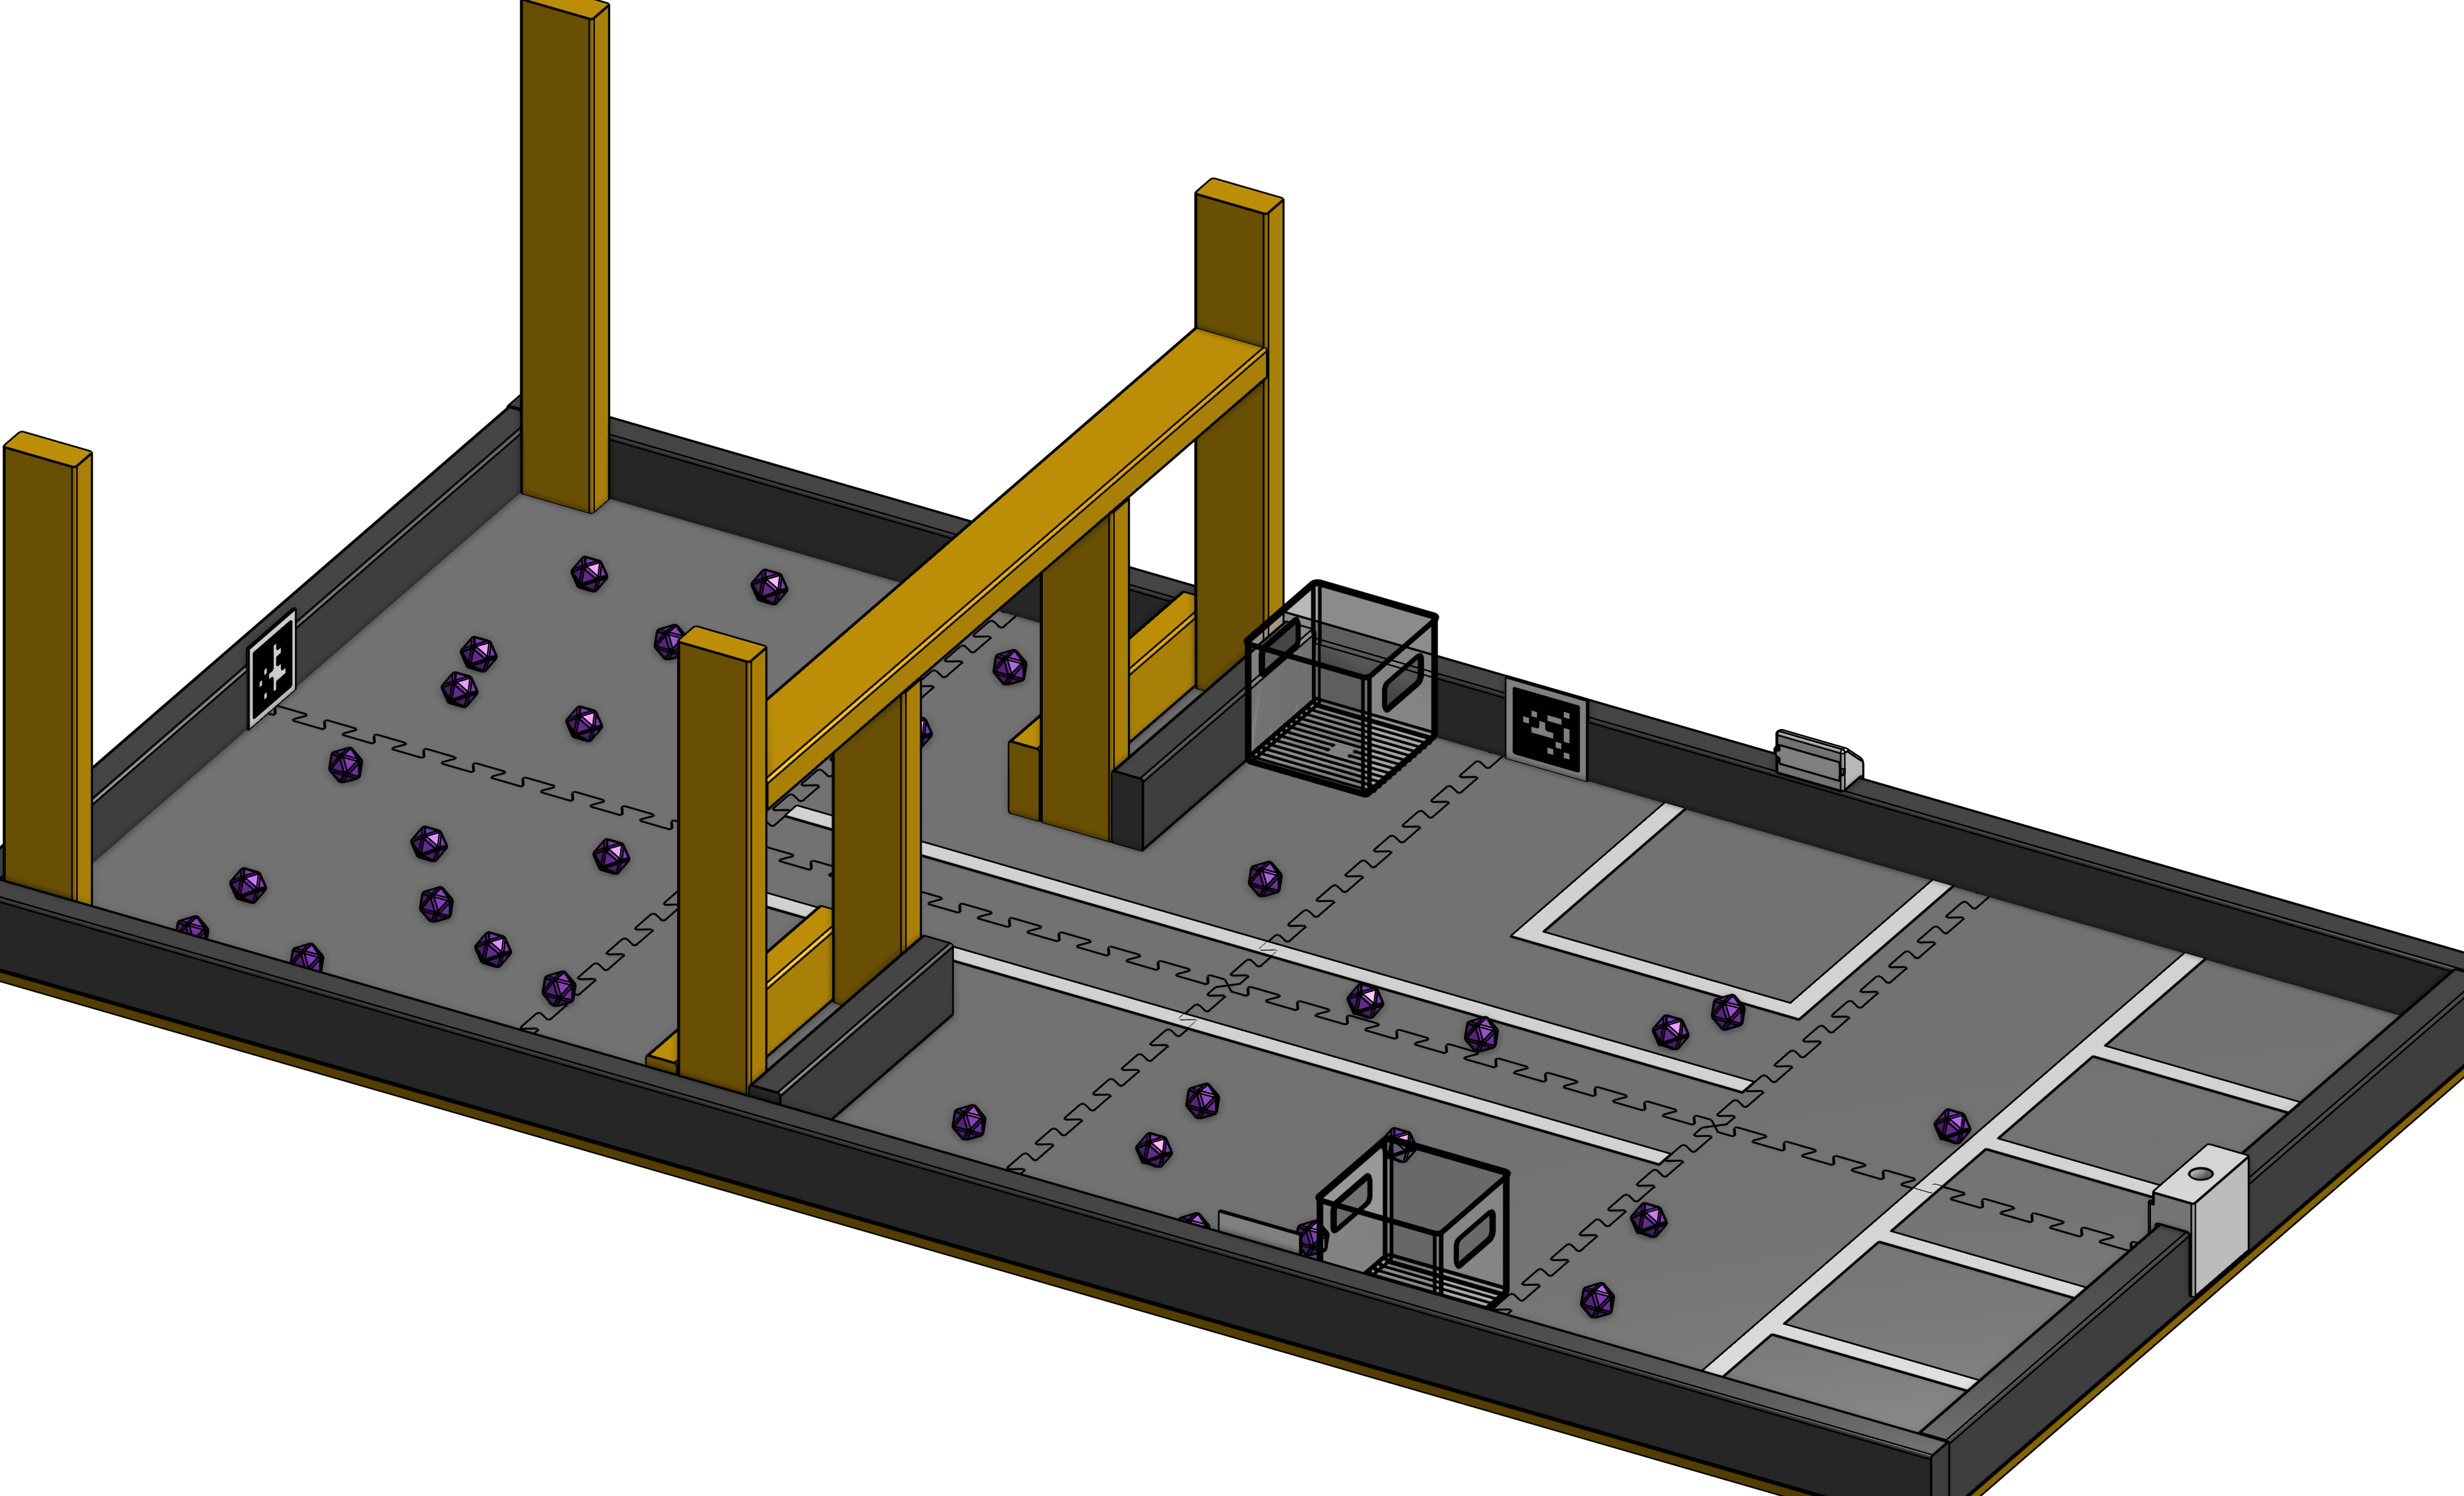
\includegraphics[width=20.0cm]{Mining Mayhem Field Opposite Corner.png}
      \caption{Game Field to compete on.}
    \end{figure}

  \end{block}
 
    % \begin{figure}
    %   \centering
    %   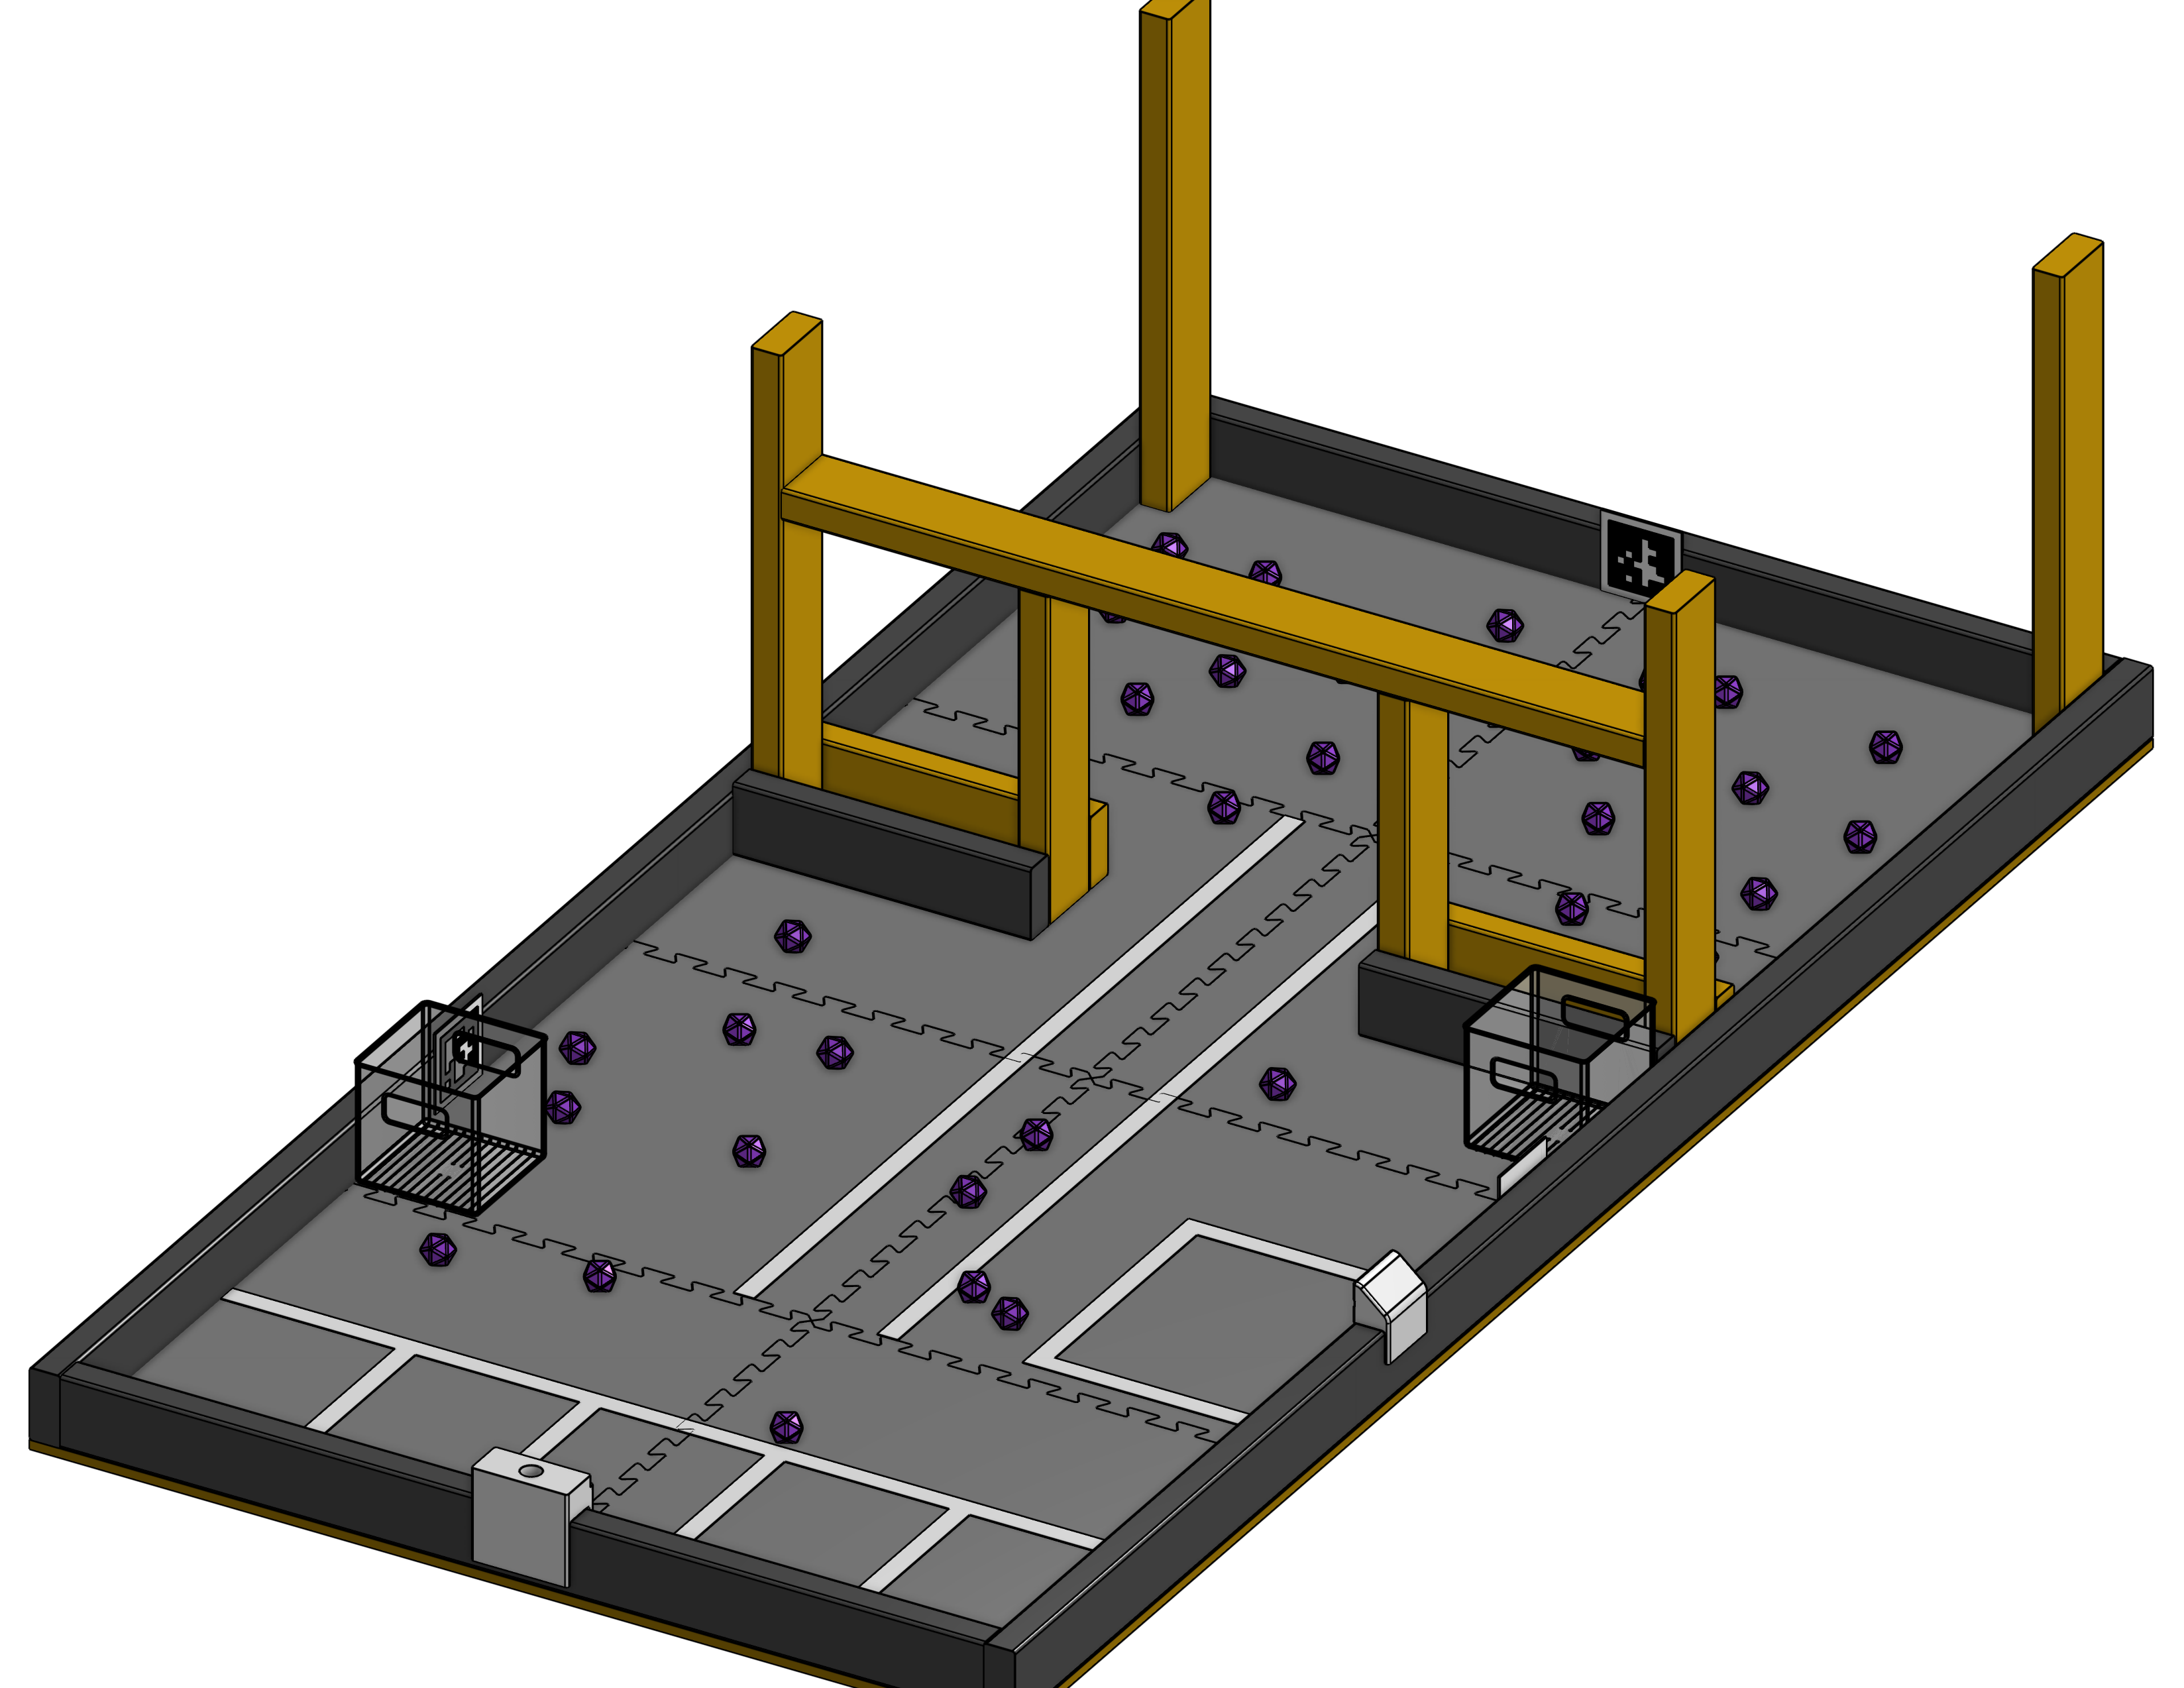
\includegraphics[width=20.0cm]{Mining Mayhem Field.png}
    %   \caption{Game Field to compete on.}
    % \end{figure}

\end{column}

\separatorcolumn

\begin{column}{\colwidth}

    \begin{figure}
      \centering
      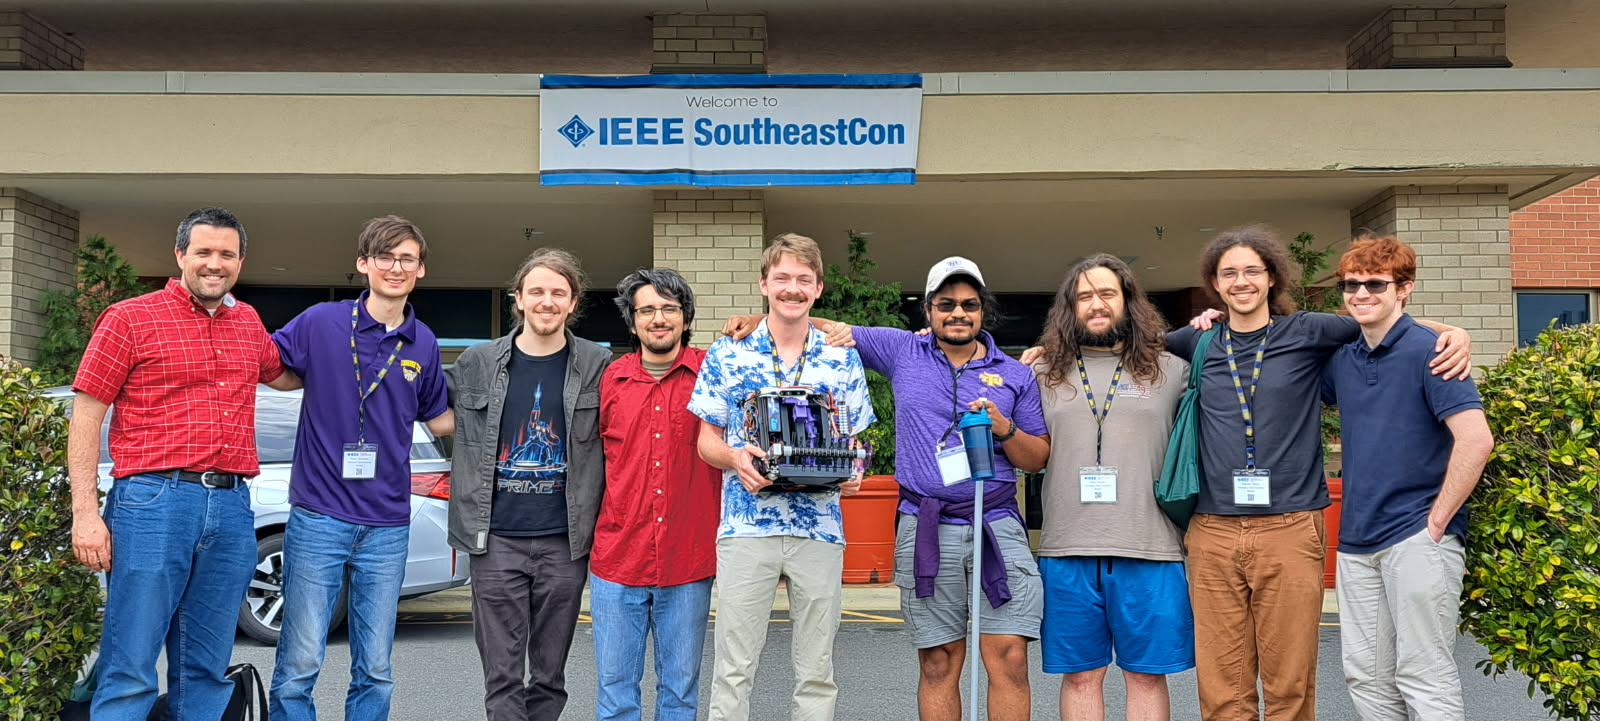
\includegraphics[width=30.0cm]{Team Picture SECON 2025.jpg}
      \caption{Micah Rentschler, Sean Borchers, Caleb Sullivan, Alex Cruz, Cooper Nelson, Phoenix Sims, Sam Hunter, Dakota Moye, Nick Moulton}
    \end{figure}

    \begin{block}{Design}
    \begin{itemize}
    
      \item \textbf{Navigation}
        \begin{itemize}
          \item The robot navigates along a predetermined path intended to maximize points based on the problem described in the introduction. To facilitate this goal, this subsystem sends commands to the motor control subsystem that are constructed, based on the feedback from the sensor and camera subsystems, to ensure accurate movement.
        \end{itemize}
        
      \item \textbf{Motor Control}
        \begin{itemize}
          \item The motor control subsystem includes the design and operation of the motors for the robot wheels, arms, and other mechanisms that move based on sensor input and navigational commands. This subsystem would be considered lower-level robot control, as it explicitly includes details about certain motor speeds and directions for when specific conditions are met during play.
        \end{itemize}
      
      \item \textbf{Camera}
        \begin{itemize}
          \item The camera detects objects and symbols.
        \end{itemize}
      
      \item \textbf{Sensors}
        \begin{itemize}
          \item The sensors subsystem is able to detect orientation, magnetic fields, and light levels. This information is then provided to the controllers for processing. Orientation sensor provides information about the robot's current position and which way it is facing. The magnetic sensors detect if there is a magnetic field in specific materials. The light sensors detect a difference in light levels.
        \end{itemize}
    
    \end{itemize}

    \begin{figure}
      \centering
      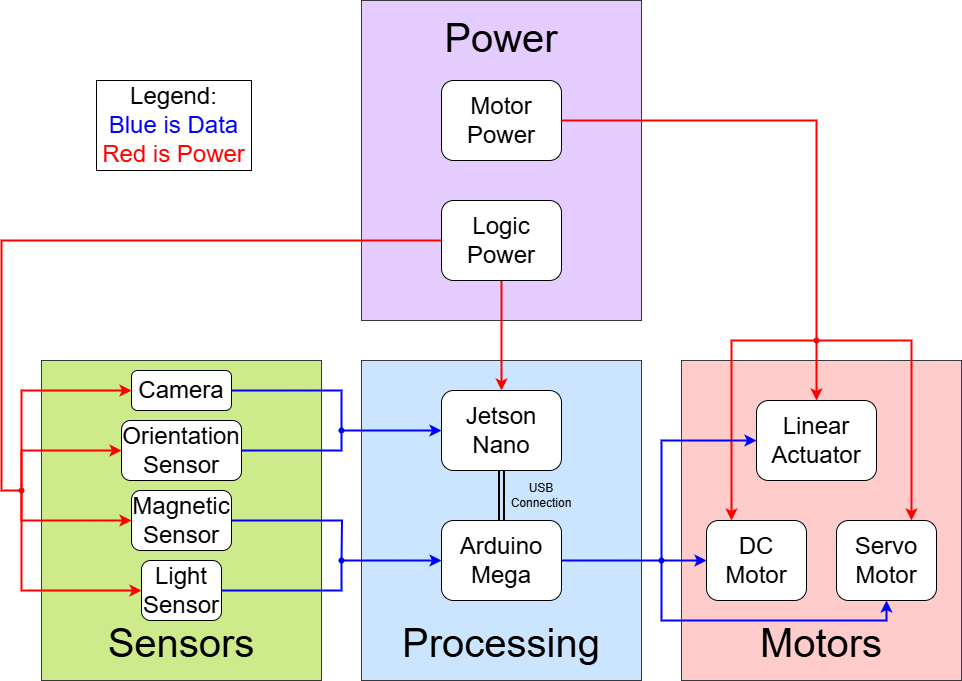
\includegraphics[width=20.0cm]{High_Block_Diagram.png}
      \caption{High Level Block Diagram.}
    \end{figure}
  
  \end{block}

\end{column}

\separatorcolumn

\begin{column}{\colwidth}

    \begin{block}{Experimentation}
    \item \textbf{Capabilities}
        \begin{itemize}
          \item The robot can start within a 12x12x12 inch space and expand upon activating a start LED.
          \item The robot can navigate autonomously by translational and rotational motion.
          \item The robot can sweep material at its front and send it up an auger for sorting.
          \item The robot can pick up and carry containers used for the material.
          \item The robot can hold a beacon and place it at a position along the field wall (as seen in the middle of the shorter wall in Figure 1).
        \end{itemize}

    \begin{figure}
      \centering
      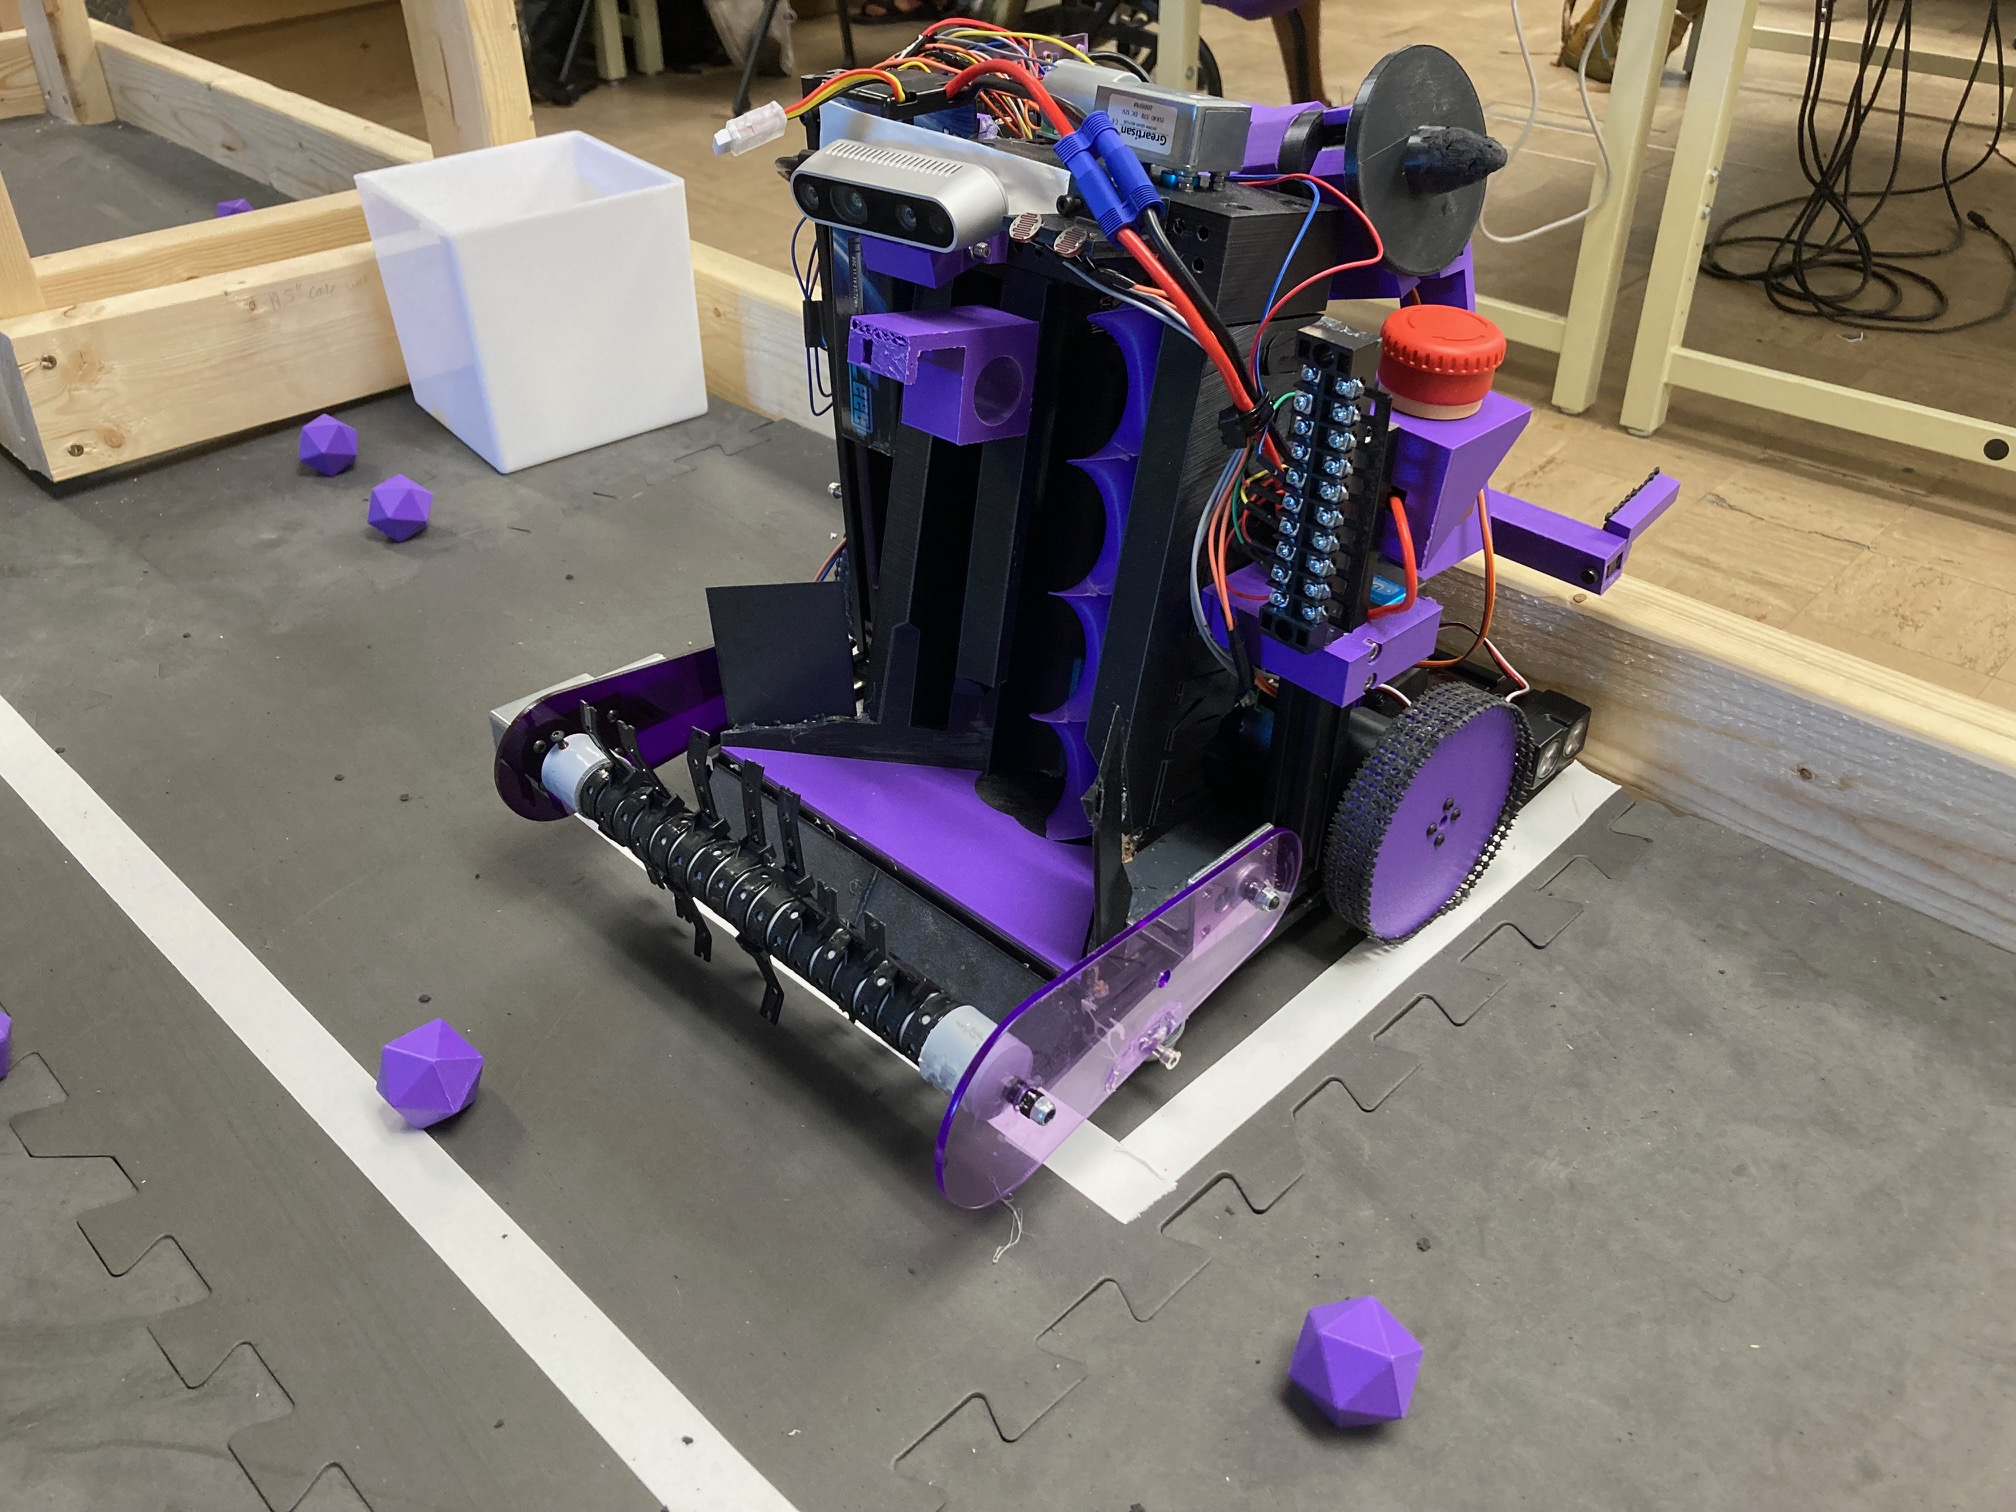
\includegraphics[width=20.0cm]{Robot_Practice_Field.jpg}
      \caption{Final Robot Product}
    \end{figure}

  \end{block}


  \begin{block}{Conclusion}
    The goal of the design process was to focus on reliably obtaining points, and conduct an extensive testing period. Complications in the design of the physical robot led to a lacking development period and a lack of a testing period. Although, during testing, the robot could obtain enough points to pass the first round of the competition, it could only do this unreliably. During the competition, the robot failed to start twice which led to its elimination.

    We would like to thank Micah Rentschler, Dr. Syed Ali Asad Rizvi, our mechanical engineering counterpart, the College of Engineering, and IEEE SECON for their guidance, support, and the ability to work on such a memorable project.


  \begin{columns}[t]
  
    \begin{column}{0.3\colwidth}
      \begin{table}[ht]
        \begin{center}
          % \caption{Bill of Materials}
          \label{tab:InitialECEBillofMaterials}
          \rowcolors{2}{gray!10}{gray!20}
          \begin{tabular}{l|r} % <-- Alignments: 1st column left and 2nd middle right, with vertical lines in between
            \toprule
            \multicolumn{2}{c}{\textbf{Initial ECE Bill of Materials}} \\
            \midrule
            \cellcolor{white}\textbf{Subsystem} & \cellcolor{white}\textbf{Cost} \\
            \midrule
            Navigation & \$260 \\
            Motor Control & \$180 \\
            Camera & \$272 \\
            Sensors & \$550 \\
            Power & \$332 \\
            \cellcolor{white}\textbf{Total} & \cellcolor{white}\$1594 \\
            \bottomrule
          \end{tabular}
        \end{center}
      \end{table}    
    \end{column}

    
    \begin{column}{0.3\colwidth}
      \begin{table}[ht]
        \begin{center}
          % \caption{Bill of Materials}
          \label{tab:FinalECEBillofMaterials}
          \rowcolors{2}{gray!10}{gray!20}
          \begin{tabular}{l|r} % <-- Alignments: 1st column left and 2nd middle right, with vertical lines in between
            \toprule
            \multicolumn{2}{c}{\textbf{Final ECE Bill of Materials}} \\
            \midrule
            \cellcolor{white}\textbf{Subsystem} & \cellcolor{white}\textbf{Cost} \\
            \midrule
            Navigation & \$304.97 \\
            Motor Control & \$189.44 \\
            Camera & \$309.67 \\
            Sensors & \$106.92 \\
            Power & \$114.72 \\
            \cellcolor{white}\textbf{Total} & \cellcolor{white}\$1025.72 \\
            \bottomrule
          \end{tabular}
        \end{center}
      \end{table}    
    \end{column}


    \begin{column}{0.3\colwidth}
      \begin{table}[ht]
        \begin{center}
          % \caption{Bill of Materials}
          \label{tab:RobotTotalBillofMaterials}
          \rowcolors{2}{gray!10}{gray!20}
          \begin{tabular}{l|r} % <-- Alignments: 1st column left and 2nd middle right, with vertical lines in between
            \toprule
            \multicolumn{2}{c}{\textbf{Robot Total Bill of Materials}} \\
            \midrule
            \cellcolor{white}\textbf{Subsystem} & \cellcolor{white}\textbf{Cost} \\
            \midrule
            Electrical Components & \$1025.72 \\
            Mechanical Components & \$1015.35 \\
            \cellcolor{white}\textbf{Total} & \cellcolor{white}\$2041.07 \\
            \bottomrule
          \end{tabular}
        \end{center}
      \end{table}    
    \end{column}


  \end{columns}

  \end{block}

\end{column}

\separatorcolumn
\end{columns}
\end{frame}

\end{document}
